\chapter{Proof of Concept}%
\label{ch:proofofconcept}

Doorheen dit hoofdstuk volgt een toelichting omtrent het uitbouwen van de POC die zal gevalideerd worden tegenover een commercieel beschikbaar alternatief zoals besproken in het voorgaande hoofdstuk. Voor het uitbouwen van deze applicatie is de keuze genomen om dit in Kotlin met behulp van Android Studio te ondernemen. Dit heeft als nadeel dat het de app beperkt tot 1 specifiek platform maar dit heeft dan als positief gevolg dat er meer informatie kan verzameld worden vanuit het toestel vanwege de aanwezigheid van specifieke functies die toegang hebben tot het toestel. Hierna volgt een diepere kijk omtrent het doel van dit project en de effectieve uitwerking alsook de uitkomst hiervan. 

\section{Doelstelling en requirements}

Het doel van de POC is een uitwerking van de applicatie die kan gebruikt worden door een student of andere medewerker om zo op een eenvoudige en herhaalbare manier een opgezet netwerk te onderwerpen aan een veelvoud van testen. In de komende hoofdstukken zal toegelicht worden hoe deze applicatie tot stand is gekomen alsook een korte introductie in hoe deze er visueel uitziet en informatie omtrent de werking hiervan. 

\section{Uitwerking}

De uitwerking werd gespreid over meerdere weken waarin een applicatie tot stand kwam. Deze iteraties waren periodes van 2 weken met duidelijke doelen voor elke iteratie. Tussen de meerdere iteraties lag een nadruk op terugkoppelen naar de verscheidene doelgroepen om de bruikbaarheid relevant te houden met het ontwikkelingsproces. 

\subsection{Werking van de applicatie}

\subsection{Opstart applicatie}

Wanneer een gebruiker de applicatie voor het eerst opstart komt men op onderstaand scherm terecht. Hier is het de bedoeling dat men aangeeft tot welk team ze behoren en voor welk project dit nodig is. Een database houd deze waarden bij. Dit kan dan meegestuurd worden naar een database om zo een duidelijker onderscheid te maken tussen verscheidene waarden die mogelijks gelijktijdig binnen komen. 

\begin{figure}[!htb]
    \includegraphics[width=0.3\linewidth]{graphics/startscreen}
    \caption[Scherm waar eindgebruiker bij uitkomt gedurende eerste opstart]{Scherm waar eindgebruiker bij uitkomt gedurende eerste opstart}
    \label{fig:startscreen}
\end{figure}

\subsection{Startscherm}

Na de initiële opstart en het toekennen van permissies komt men bij het scherm hieronder uit. Hier ziet men met welk type netwerk, in dit specifiek geval Wifi of een cellulaire verbinding, men huidig mee verbonden is en welk IP-adres of URL er naar gepingd zal worden gedurende de test fase. Deze informatie en configuratie is van belang vanwege het feit dat dit een zware impact kan hebben op de mogelijk verkregen resultaten.

\begin{figure}[!htb]
    \includegraphics[width=0.3\linewidth]{graphics/homescreen}
    \caption[Scherm van waaruit de eindgebruiker na opzet testen kan starten]{Scherm van waaruit de eindgebruiker na opzet testen kan starten}
    \label{fig:homescreen}
\end{figure}

\subsection{Continue test omgeving}

Dit scherm volgt direct op het hiervoor besproken deel en integreert de functionaliteit om een netwerk te onderwerpen aan een ping test. Dit heeft geen eindtijd en gebeurt standaard met een interval van 1 seconde, en neemt een zelfgekozen route naar het opgegeven IP adres. Deze parameters staan beide open voor aanpassingen zonder dat het de test onderbreekt. Ook heeft de eindgebruiker een keuze omtrent het starten van een specifieke testroutine of om de data die verzameld is door te sturen naar een externe database. 

\begin{figure}[!htb]
    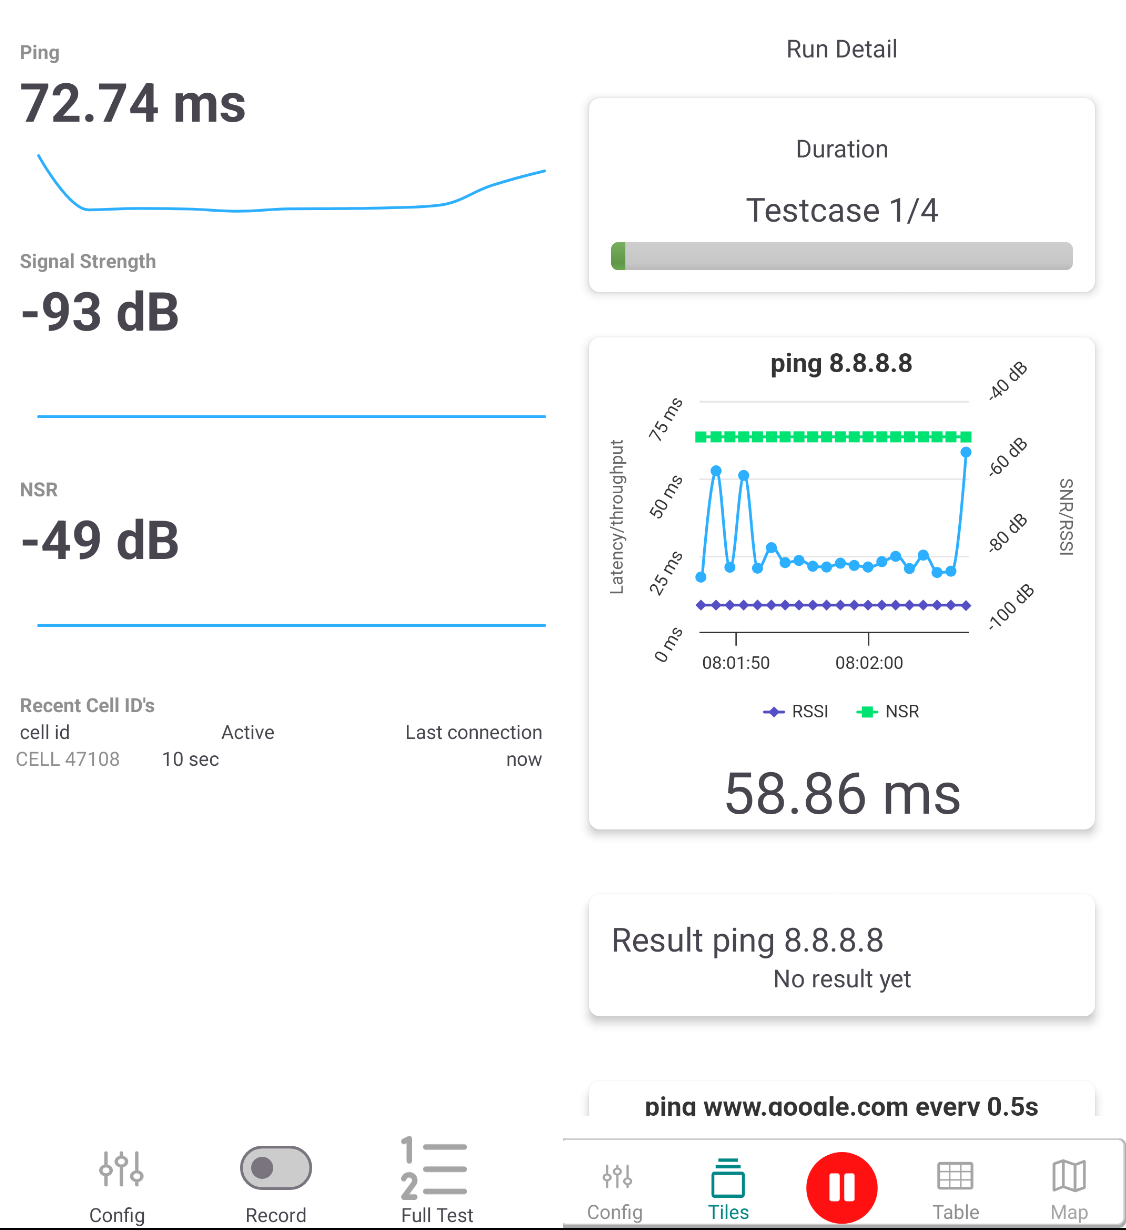
\includegraphics[width=1\linewidth]{graphics/continuousspecificmerge}
    \caption[Links het scherm van een eindeloze ping test en rechts een specifieke test die uitgevoerd wordt.]{Links het scherm van een eindeloze ping test en rechts een specifieke test die uitgevoerd wordt.}
    \label{fig:continuousandspecific}
\end{figure}

\subsection{Vervullen specifieke test}

Er is een mogelijkheid tot het uitvoeren van specifieke testen, deze opgenomen in de proof-of-concept zijn een reeks van aangepaste ping testen en een test om de download en upload snelheid te kunnen registreren. Deze waarden bevatten automatisch de locatie van de eindgebruiker en worden standaard verstuurd naar een externe locatie voor analyse. Deze diepgaandere testen bevatten ook verscheidene andere mogelijkheden om deze data weer te geven zoals een tabel of kaart in plaats van de generieke grafieken.

\section{Test opstelling}

G-NetTrack Pro en de POC werden beiden ingezet om een netwerk opgezet door Citymesh te onderwerpen aan testen. Dit in kwestie was dat aanwezig op Graspop Metal Meeting 2024 waar er connectiviteit was voorzien om er voor te zorgen dat alle contactloze betaalpunten operationeel bleven. Deze opstelling bestond uit meerdere cellen om er zo voor te zorgen dat elk deel van het terrein wel bereikt kon worden. Belangrijkste functionaliteit voor deze bussiness case was dat een apparaat verbonden was dus bleek latentie belangrijk dan up- en download snelheden. 